% This file was created by matlab2tikz.
%
%The latest updates can be retrieved from
%  http://www.mathworks.com/matlabcentral/fileexchange/22022-matlab2tikz-matlab2tikz
%where you can also make suggestions and rate matlab2tikz.
%
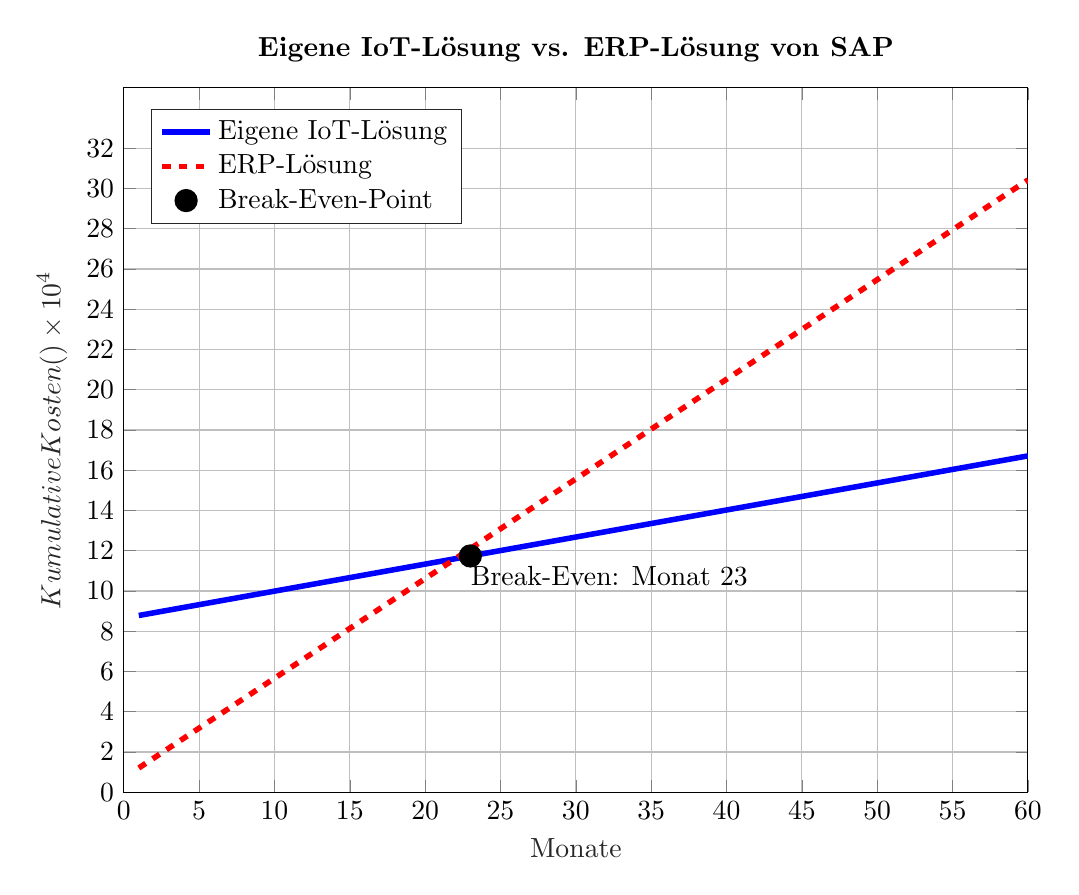
\begin{tikzpicture}

\begin{axis}[%
width=4.521in,
height=3.522in,
at={(0.758in,0.525in)},
scale only axis,
xmin=0,
xmax=60,
xlabel style={font=\color{white!15!black}},
xlabel={Monate},
ymin=0,
ymax=35,
ytick={ 0,  2,  4,  6,  8, 10, 12, 14, 16, 18, 20, 22, 24, 26, 28, 30, 32},
ylabel style={font=\color{white!15!black}},
ylabel={$\text{Kumulative Kosten (€) }\times\text{ 10}^\text{4}$},
axis background/.style={fill=white},
title style={font=\bfseries},
title={Eigene IoT-Lösung vs. ERP-Lösung von SAP},
xmajorgrids,
ymajorgrids,
legend style={at={(0.03,0.97)}, anchor=north west, legend cell align=left, align=left, draw=white!15!black}
]
\addplot [color=blue, line width=2.0pt]
  table[row sep=crcr]{%
1	8.7839\\
2	8.9183\\
3	9.0527\\
4	9.1871\\
5	9.3215\\
6	9.4559\\
7	9.5903\\
8	9.7247\\
9	9.8591\\
10	9.9935\\
11	10.1279\\
12	10.2623\\
13	10.3967\\
14	10.5311\\
15	10.6655\\
16	10.7999\\
17	10.9343\\
18	11.0687\\
19	11.2031\\
20	11.3375\\
21	11.4719\\
22	11.6063\\
23	11.7407\\
24	11.8751\\
25	12.0095\\
26	12.1439\\
27	12.2783\\
28	12.4127\\
29	12.5471\\
30	12.6815\\
31	12.8159\\
32	12.9503\\
33	13.0847\\
34	13.2191\\
35	13.3535\\
36	13.4879\\
37	13.6223\\
38	13.7567\\
39	13.8911\\
40	14.0255\\
41	14.1599\\
42	14.2943\\
43	14.4287\\
44	14.5631\\
45	14.6975\\
46	14.8319\\
47	14.9663\\
48	15.1007\\
49	15.2351\\
50	15.3695\\
51	15.5039\\
52	15.6383\\
53	15.7727\\
54	15.9071\\
55	16.0415\\
56	16.1759\\
57	16.3103\\
58	16.4447\\
59	16.5791\\
60	16.7135\\
};
\addlegendentry{Eigene IoT-Lösung}

\addplot [color=red, dashed, line width=2.0pt]
  table[row sep=crcr]{%
1	1.2068\\
2	1.702\\
3	2.1972\\
4	2.6924\\
5	3.1876\\
6	3.6828\\
7	4.178\\
8	4.6732\\
9	5.1684\\
10	5.6636\\
11	6.1588\\
12	6.654\\
13	7.1492\\
14	7.6444\\
15	8.1396\\
16	8.6348\\
17	9.13\\
18	9.6252\\
19	10.1204\\
20	10.6156\\
21	11.1108\\
22	11.606\\
23	12.1012\\
24	12.5964\\
25	13.0916\\
26	13.5868\\
27	14.082\\
28	14.5772\\
29	15.0724\\
30	15.5676\\
31	16.0628\\
32	16.558\\
33	17.0532\\
34	17.5484\\
35	18.0436\\
36	18.5388\\
37	19.034\\
38	19.5292\\
39	20.0244\\
40	20.5196\\
41	21.0148\\
42	21.51\\
43	22.0052\\
44	22.5004\\
45	22.9956\\
46	23.4908\\
47	23.986\\
48	24.4812\\
49	24.9764\\
50	25.4716\\
51	25.9668\\
52	26.462\\
53	26.9572\\
54	27.4524\\
55	27.9476\\
56	28.4428\\
57	28.938\\
58	29.4332\\
59	29.9284\\
60	30.4236\\
};
\addlegendentry{ERP-Lösung}

\addplot [color=black, only marks, mark size=4.0pt, mark=*, mark options={solid, fill=green, black}]
  table[row sep=crcr]{%
23	11.7407\\
};
\addlegendentry{Break-Even-Point}

\node[below right, align=left, inner sep=0]
at (axis cs:23,11.241) {Break-Even: Monat 23};
\end{axis}
\end{tikzpicture}%